\begin{figure}[!htbp]
\centering
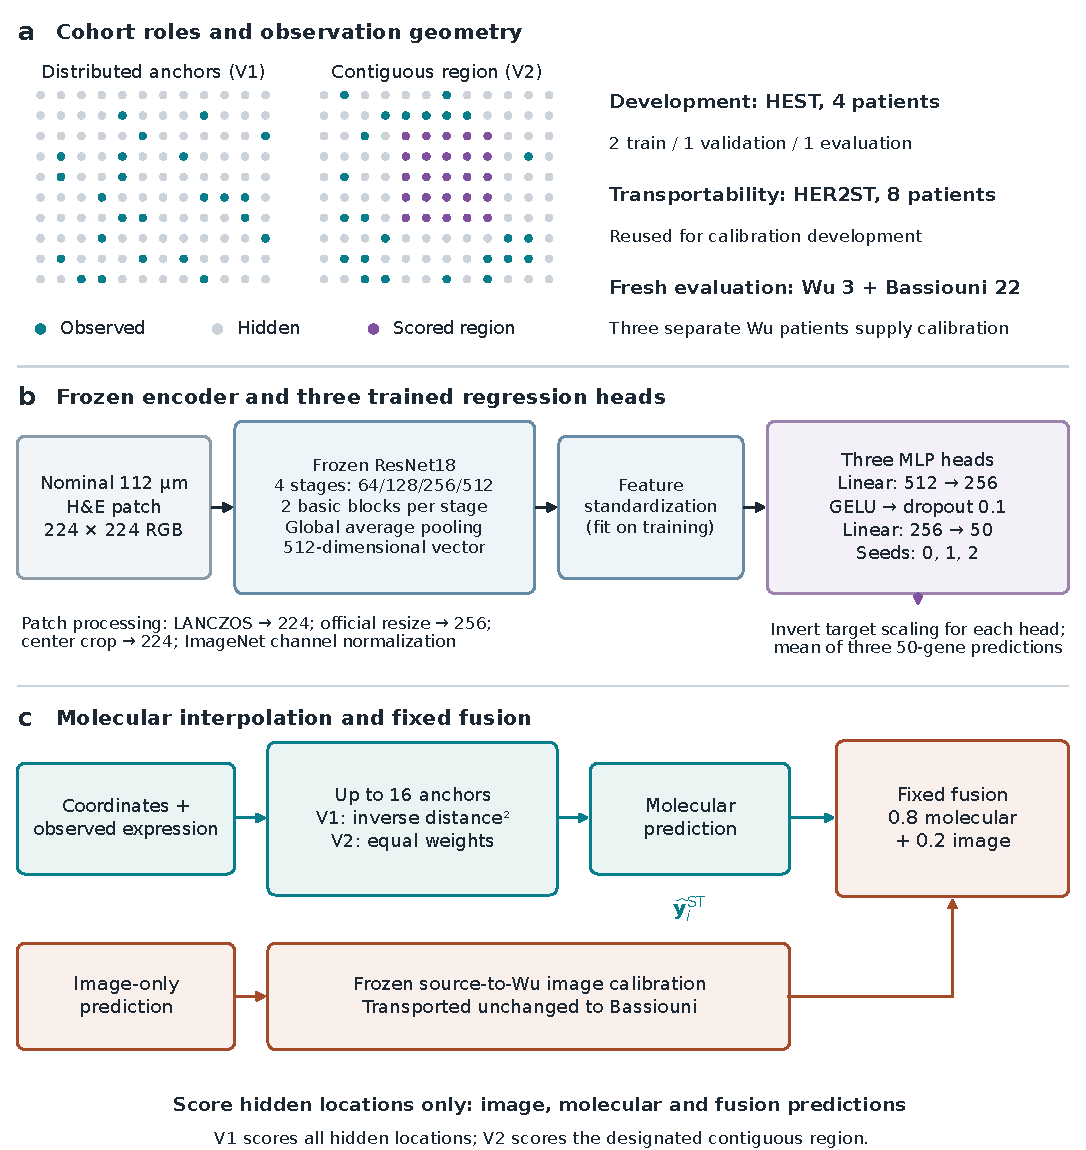
\includegraphics[width=\textwidth,height=0.72\textheight,keepaspectratio]{figures/Figure1.pdf}
\caption{\textbf{Original study design and neural-image/molecular reconstruction architecture.} \textbf{a,} Cohort roles and illustrative observation geometries. Teal locations are observed molecular anchors; gray locations are hidden; purple locations form the contiguous scored region. The synthetic spatial examples illustrate 20\% coverage and are not patient measurements. The Wu calibration and evaluation groups contain different patients. \textbf{b,} The frozen ImageNet ResNet18 maps histology to a 512-dimensional vector after global average pooling; the ImageNet classifier is removed. External nominal 112-\um{} patches are first resized to $224\times224$ with LANCZOS, then processed by the official resize-to-256, central-crop-to-224 and channel-normalization transform. Feature scaling fitted on the training patients precedes each $512\rightarrow256\rightarrow50$ MLP, with GELU activation and dropout 0.1 after the hidden linear layer. The three heads use seeds 0, 1 and 2. Their predictions are inverse-scaled to the common target units and averaged. \textbf{c,} Molecular interpolation uses up to 16 observed neighbors, with inverse-distance-squared weighting for distributed evaluation (V1) and equal weighting for contiguous regional completion (V2). Fixed fusion combines this output with the calibrated image prediction using weights 0.8 and 0.2. The uncalibrated image ensemble is also evaluated separately. Calibration uses the development-training and Wu calibration patients and is transported unchanged to Bassiouni. Evaluation uses hidden locations only. V1 and V2 differ in weighting and scoring support as well as observation geometry.}
\label{fig:overview}
\end{figure}
